\subsection{Satz}
Seien $n \in \N , k_1,...k_d \in \N_0,~ k_1+...+k_d=n $

Gegeben seien d verschiedene Sorten von Objekten, jeweils $k_i$ identische von Sorte $i, i=1,...,d$

Die Anzahl der Möglichkeiten diese $k_1+...+k_d = n$ Objekte auf n Plätzen anzuordnen, ist:

$$ \frac{n!}{k_1!*k_2!*...*k_d!}$$ 

\subsubsection*{Beweis:}
Wähle $k_1$, der n Plätze für Objekte vom Typ 1 aus $\binom{n}{k_1}$ Möglichkeiten

Wähle $k_2$, der übrigen $n-1$ für Objekte vom Typ 2 aus $\binom{n-1}{k_2}$ Möglichkeiten

Wähle $k_3$, der übrigen $n-2$ für Objekte vom Typ 3 aus $\binom{n-2}{k_3}$ Möglichkeiten


.

.

.


Das liefert: $\binom{n}{k_1}\binom{n-k_1}{k_2}...\binom{n-k_1-...k_d-1}{k_d} = \frac{n!}{k_1!(n-k_1)!}*\frac{(n-k_1)!}{k_1!(n-k_1-k_2)!}*\frac{(n-k_1)!}{k_2!(n-k_1-k_2)!}*...*\frac{(n-k_1-...-k{d-1})!}{k_d!((n-k_1-...-k{d})!)}) $

$= \frac{n!}{k_1!*k_2!*...*k_d!}$ Möglichkeiten.

\subsection{Definition}
Sei $n \in \N, k_1,...,k_d \in \N_0,~ k_1+...+k_d = n$

Der \underline{Multinomialkoeffizient} $\binom{n}{k_1,k_2,...,k_d}$ ist derfiniert durch

$$\binom{n}{k_1,k_2,...,k_d} := \frac{n!}{k_1!k_2!...k_d!} $$

Beachte: $\binom{n}{k} = \binom{n}{k,n-k}$

Bezeichnung stammt vom \underline{Multinomialsatz:}

$x_1,...,x_d \in \R,$ so $(x_1+...+x_d)^n= \sum_{k_i \in \N}\binom{n}{k_1,k_2,...,k_d}x_1^{k_1}x_2^{k_2}...x_d^{k_d}$

\section{Linerare Rekursion}
\subsection{Definition}
\begin{enumerate}
	\item Eine \underline{Rekursion} ist ein unendliches System von Gleichungen der Form
	
	\begin{itemize}
		\item[($*)$] $x_n = f_n(x_{n-1,x_1})$ für alle $n\geq \underbrace{n_0}_{fest} $
		
		($f_n$ ist berechenbare Funktion)
		
	\end{itemize}
	Bei Vorgabe von beliebiger \underline{Anfangswerten} $x_1 = a_1,...,x_{n_0-1}=a_{n_0-1}$ sind $ a_{n_0}= f_{n_0-1}( a_{n_0-1},...,a_{1}), a_{n_0+1}= f_{n_0+1}(a_{n_0},a_{n_0-1},...,a_{1}),...$ festgelegt.
	
	Jede Folge $(x_1,x_2,...)$ von Elementen aus $\R$(oder $\C$), die $(*)$ erfüllt, heißt Lösung der Rekursion.
	
	\subsubsection*{Beispiel:}
	x$_n= x_{n-1}^2+2x_{n-2}x_1$ für n$\geq$ 3
	
	Anfangswerte: $a_1=1,~ a_2=2$
	
	$a_3 = a_2^2+2a_1^2=6$
	
	$a_4 = a_3^2+2a_2a_1=40$
	
	\item Eine \underline{Rekursion k-ter Ordnung:}
	
	$x_n=f_n(x_{n-1},...,x_{n-k}) $ für alle $n\geq k+1$
	
	\item Eine Rekursion heißt \underline{linear von Ordnung k mit sonstanten Koeffizienten}, falls
	
	$x_n= c_1x_{n-1}+c_2x_{n-2}+...+c_kx_{n-k} +g(n)$ für alle $ n\geq k+1$
	
	$c_1,...,c_k \in \R $(oder $\C$) fest (unabhängig von n), $c_k \neq 0$
	
	Ist $g(n)=0$ für alle $n\geq k+1$, so heißt Rekursion \underline{homogen}, ansonsten \underline{inhomogen}. 
	
\end{enumerate}

\subsection{Beispiel}
\begin{enumerate}
	\item \underline{Fibonacci-Zahlen}
	
	(Leonardo von Pisa $(*1170 ; \dagger1250$, Liber abaci)
	
	Auf wie viele Arten lässt sich $n \in \N$ als geordnete Summe von Eines und Zweien schreiben?
	
	
	\begin{tabular}{c c c}
		Anzahl $F_n$:	& $F_1=1$ 	& $1$\\
						& $f_2=2$	& $1+1,2$\\
						& $f_3=3$	& $1+1+1,1+2,2+1$\\
	\end{tabular}
	
	\begin{tabular}{c c l}
		$n\geq 3:$] 	&$\underbrace{+...+}_{n-1}+1$ & $F_n = F_{n-1}+F_{n-2}$, $F_1=1$, $F_2=2$\\
						&$\underbrace{+...++}_{n-2}+2$ &$F_4 = F_3+F_2 = 5$\\
						&								& lineare Rekursion mit konst. Koeff. Ordnung. 2, homogen 
	\end{tabular}
	\subsection*{Anderes Beispiel}
	Wie viele $0-1-$Folgen der Länge $n$ gibt es ohne zwei aueinanderfolgende Nullen?
	
	$a_1=2, a_2=3$
	
	$n\geq 3:$ $\overbrace{.......}^{a_{n-1}}1$ $a_n = a_{n-1}+a_{n-2}$ Fibonacci-Rekursion \quad $a_n=F_{n+1}$
	
	\qquad \quad $\overbrace{.......}^{a_{n-2}}10$
	 
	 
	 \item \underline{Türme von Hanoi}
	 \begin{center}
		 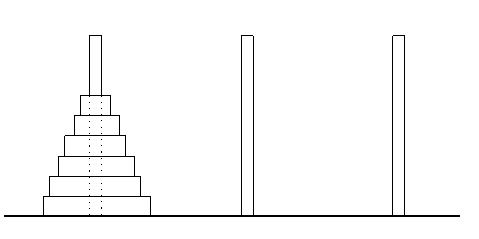
\includegraphics{hanoi.jpg}
	 \end{center}

	 3 Stäbe, n verschieden große Scheiben, auf Stab 1, der Größe nach geordnet, größte unten.
	 
	 Scheiben auf Stab 2 legen, in derselben Anordnung.
	 \begin{itemize}
	 	\item In jedem Zug 1 Scheibe umlegen
	 	\item Nie darf größere Scheibe auf kleinerer liegen
	 \end{itemize}
	 $a_n$ = Mindestanzahl von Zügen Stab 1 $\rightarrow$ Stab 2
	 
	 $a_1$ = 1
	 
	 obere $n-1$ Scheiben von Stab 1 $\rightarrow$ Stab 3 $\Rightarrow$ $a_n-1$ 
	 
	 größte Scheibe von Stab 1 $\rightarrow$ Stab 2 $\Rightarrow$ 1 
	 
	 alle Scheiben von Stab 3 $\rightarrow$ Stab 2 $\Rightarrow$ $a_{n-1}$ 
	 
	 \framebox[1\width]{$a_n = 2a_{n-1}+1$}, $n\geq2, a_1 = 1$ 
	 
	 linear, Ordnung. 1, inhomogen
	 
	 \item Verallg. von b) Divide-and-Conquer-Algorithmen:
	 
	 Zerlege Problem mit Inputgröße n in a Teilprobleme kleinerer Größe, z.B. $n - 1$,
	 
	 Max. Aufwand: $T(n) = a*T(n-1)+g(n)$
	 
	 
	 \qquad   \qquad \qquad \qquad  \qquad  \qquad \qquad \qquad$\Uparrow$

	 \qquad   \qquad \qquad  \qquad  \qquad \qquad \qquad Aufwand zum Zerlegen in Teilprobleme
	 
	 \qquad   \qquad \qquad  \qquad  \qquad \qquad \qquad und zum Zusammensetzen der Teillösungen
	 
	 \qquad   \qquad \qquad  \qquad  \qquad \qquad \qquad zur Gesamtlösung.
	 
	 
\end{enumerate}